\documentclass{article}
\special{papersize=8.5in,11in}

\usepackage[lf]{electrum}
\usepackage[T1]{fontenc}
\usepackage{amsmath}
\usepackage{amsthm}
\usepackage{ulem}
\usepackage{graphicx}
\usepackage{fullpage}
\usepackage{subcaption}

\title{A Proof of the Twelve Color Theorem: \\ Hey, Nobody Bothered Before. \\ {\small Sixth Grade Class Project for Mr. Blum}}
\author{Y. T. Boveck \and Victoria V. Varg-Mack, VI}
\date{April 1$\tfrac{1}{3}$, 2071}

\begin{document}

\maketitle

\thispagestyle{empty}
\begin{center}
\begin{tabular}{p{3.9in}}
\fontfamily{cmr}\selectfont
\textit{Editor's note: Several days ago, the wreckage of a small time machine appeared in the program committee's office,
containing apparently only a copy of the proceedings from SIGBOVIK 2071.
Unfortunately, all papers but one were burnt beyond recognition.
Current speculation holds that the time machine operators forgot to disable the paradox safety interlock, and all the important (potentially causality-violating) papers were destroyed, leaving only this drivel. We're publishing it anyway, sorry.}
\end{tabular}
\end{center}

\begin{abstract}
	Roughly 100 years ago, mathematicians successfully proved the \textit{4-Color Theorem}.
	Widely regarded as one of the most important theorems in graph theory at the time, the 4-Color Theorem states that for all planar graphs there exists an assignment of colors to nobes, such that no two adjacent nobes are assigned the same color, with at most 4 colors used.
	However, modern-day computers are capable of rendering far more diverse color palettes, and the old 4-color limitation is now largely irrelevant.
	In this work we extend the old result to support 12-colorings, offer some thoughts on generalization, and leave a conspicuous hole in our proof to support our future work.
\end{abstract}

\section{Introduction}

Victoria said I had to write this section, even though she's the only one of us who actually knows how the 4-color theorem proof goes. But luckily I found a proof for the 5-color theorem that made sense, and since having more colors is obviously better, that should be even better. It goes like this:

\newtheorem{theorem}{Theorem}[section]
\newtheorem{lemma}[theorem]{Lemma}
\newtheorem{corollary}[theorem]{Corollary}
\begin{lemma}
All planar graphs have at least one vertex with at most 5 neighbors.
\end{lemma}

\begin{proof}
	Let $N(n)$ mean how many neighbors a given nobe $n$ has. Then because each edge connects two nobes, the sum of all nobes' neighbours $\sum_n N(n) = 2e$. Let's assume all nobes have at least six neighbours. Then $6n \le 2e$.

	Next let $E(f)$ mean the number of edges that make up the border of a given face $f$ of the graph. Since each edge borders 2 faces, $\sum_f E(f) = 2e$. Every region is bounded by at least 3 edges so that means $3f \le 2e$.

	If we plug all that into the ``Euler's Forumula'' that Mr. Blum gave us in class, which says that $n-e+f=2$, here's what we get: $n-e+f \le \frac{e}{3} - e + \frac{2e}{3} = 0$. But since $n-e+f = 2$ we end up with $2\le0$. Then we must have been wrong to assume all nobes have at least six neighbours. That's a ``contradiction''!
\end{proof}

\begin{theorem}
All planar graphs can be colored with no more than 5 colors so that no neighbor nobes have the same color.
\label{thm:5c}
\end{theorem}

\begin{proof}
	Let $G$ mean the graph we're trying to prove this for. Using the lemon I just proved, pick the nobe $n$ that has at most five neighbors and call those $n_1$, $n_2$, $n_3$, $n_4$, $n_5$ in whatever order you want. Let $G'$ mean the smaller graph you get by taking out $n$, which of course is still planar. Because $G'$ is smaller, we know with ``induction'' that $G'$ can be 5-colored. (That step seemed kinda weird to me but Victoria said it was legit so please don't take points off.)

	Now we're gonna assume $G$ cannot be 5-colored. For this to be true, then each $n_i$ from $1$ to $5$ must all have different colors, or else you could just pick the missing one for $n$. Let's think about the sub-graph that has only the 2 colors matching $n_1$ and $n_3$, call it $G_{13}$. If the graph is disjoint, meaning $n_1$ and $n_3$ are in two separate parts, then you would be able to re-color the graph to make $n_3$ have color $1$, so you can paint $n$ color $3$. Therefore $G_{13}$ must be connected. You can make the same argument for $G_{24}$ to be connected, but suddenly that doesn't make any sense, because a path that keeps $G_{24}$ connected would have to intersect the connected $G_{13}$!

	Therefore, even if the 5-coloring of $G'$ gives all different colors to $n_1$, $n_2$, $n_3$, $n_4$, and $n_5$, you should be able to re-color one of the $n_i$ so you can have a spare color to give to $n$. Therefore $G$ can be 5-colored.
\end{proof}


\section{The 12-Color Theorem}

\thispagestyle{empty}
In the previous section, Y.T. et al.~outlined the prior work in the field. Now we will make our main contribution; namely, to extend the 5-color theorem reviewed above to allow for 12-colorings of arbitrary planar graphs.

\begin{theorem}
	Given an arbitrary planar graph $G$, there exists an assignment of no more than 12 colors to the set of nobes $N(G)$ such that no two neighbouring nobes are assigned the same color.
\end{theorem}

\begin{proof}
	Using Theorem~\ref{thm:5c}, generate a 5-color assignment for $G$. As 5 is less than 12, this assignment suffices.
\end{proof}

\begin{corollary}
	If $G$ has at least 12 nobes, then all 12 colors may be used.
\end{corollary}

\begin{proof}
	First we will prove the case for a smaller number of colors $c<12$, by induction on $c$. Assume a graph $G$ with $c$ or more nobes, and an existing assignment of $c-1$ colors in which all colors are represented, such that $c<12$. The pigeonhole principle states that there must exist two nobes $n_1$ and $n_2$ with the same color. Simply assign the $c$th color to $n_2$ in the new coloring.

	Next for the case $c=12$. Given a graph $G$ with 12 or more nobes, there must exist an assignment of 11 colors in which all colors are represented. The pigeonhole principle states that there must exist two nobes $n_1$ and $n_2$ with the same color. Assigning the 12th color to $n_2$ causes all 12 colors to be used.
\end{proof}

An example application of our algorithm is depicted in Figure~\ref{fig:usa}.


\section{Conclusions and Future Work}

In this paper we reviewed historical developments in the field, with a particular focus on the proof of the \sout{4-Color Theorem} 5-Color Theorem; and we presented our main contribution, a constructive proof of our new \textit{12-Color Theorem} based on the assumption of existing \sout{4-colorings} 5-colorings of an arbitrary planar graph $G$.

The most significant limitation of our work is that a generalized version of our proof only applies for $C$-colorings when $C \le 12$. In future research, we plan on extending our theorem to support ever greater values of $C$. We hope the need for additional funding to study such advanced open problems is self-evident.

\newpage

\thispagestyle{empty}

\begin{figure}
	\centering
	\begin{subfigure}[b]{0.45\textwidth}
	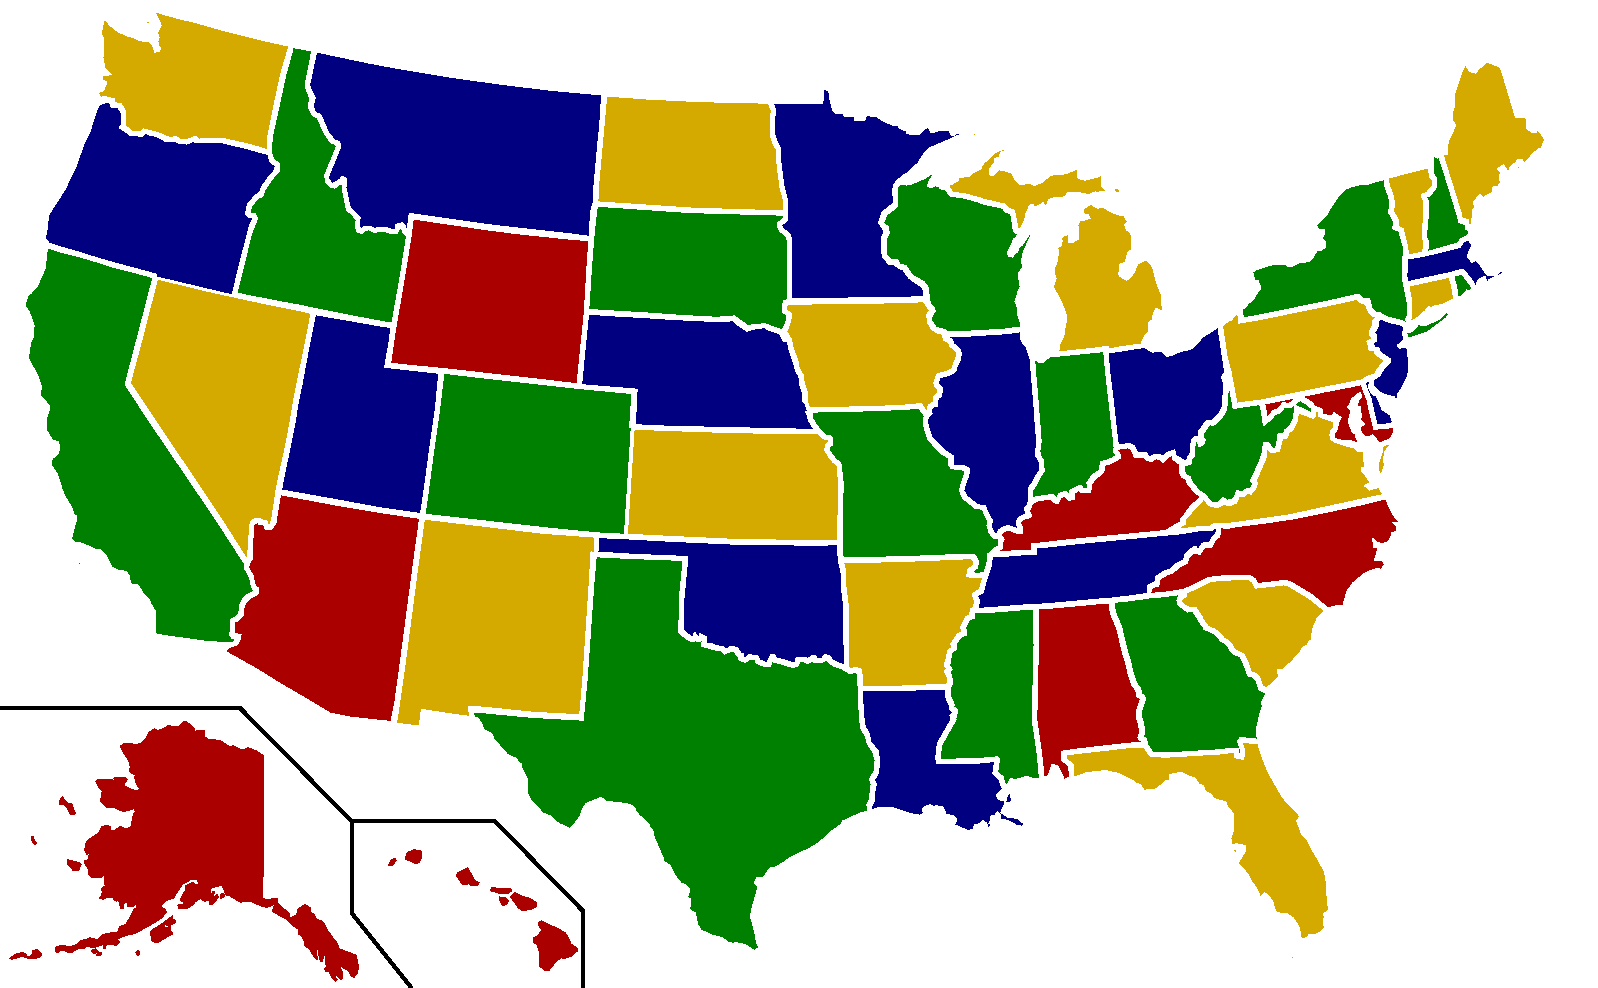
\includegraphics[width=\textwidth]{4color.pdf}
	\caption{Make a 4-color of your graph first. \\ {}}
	\end{subfigure}
	\quad
	\begin{subfigure}[b]{0.45\textwidth}
	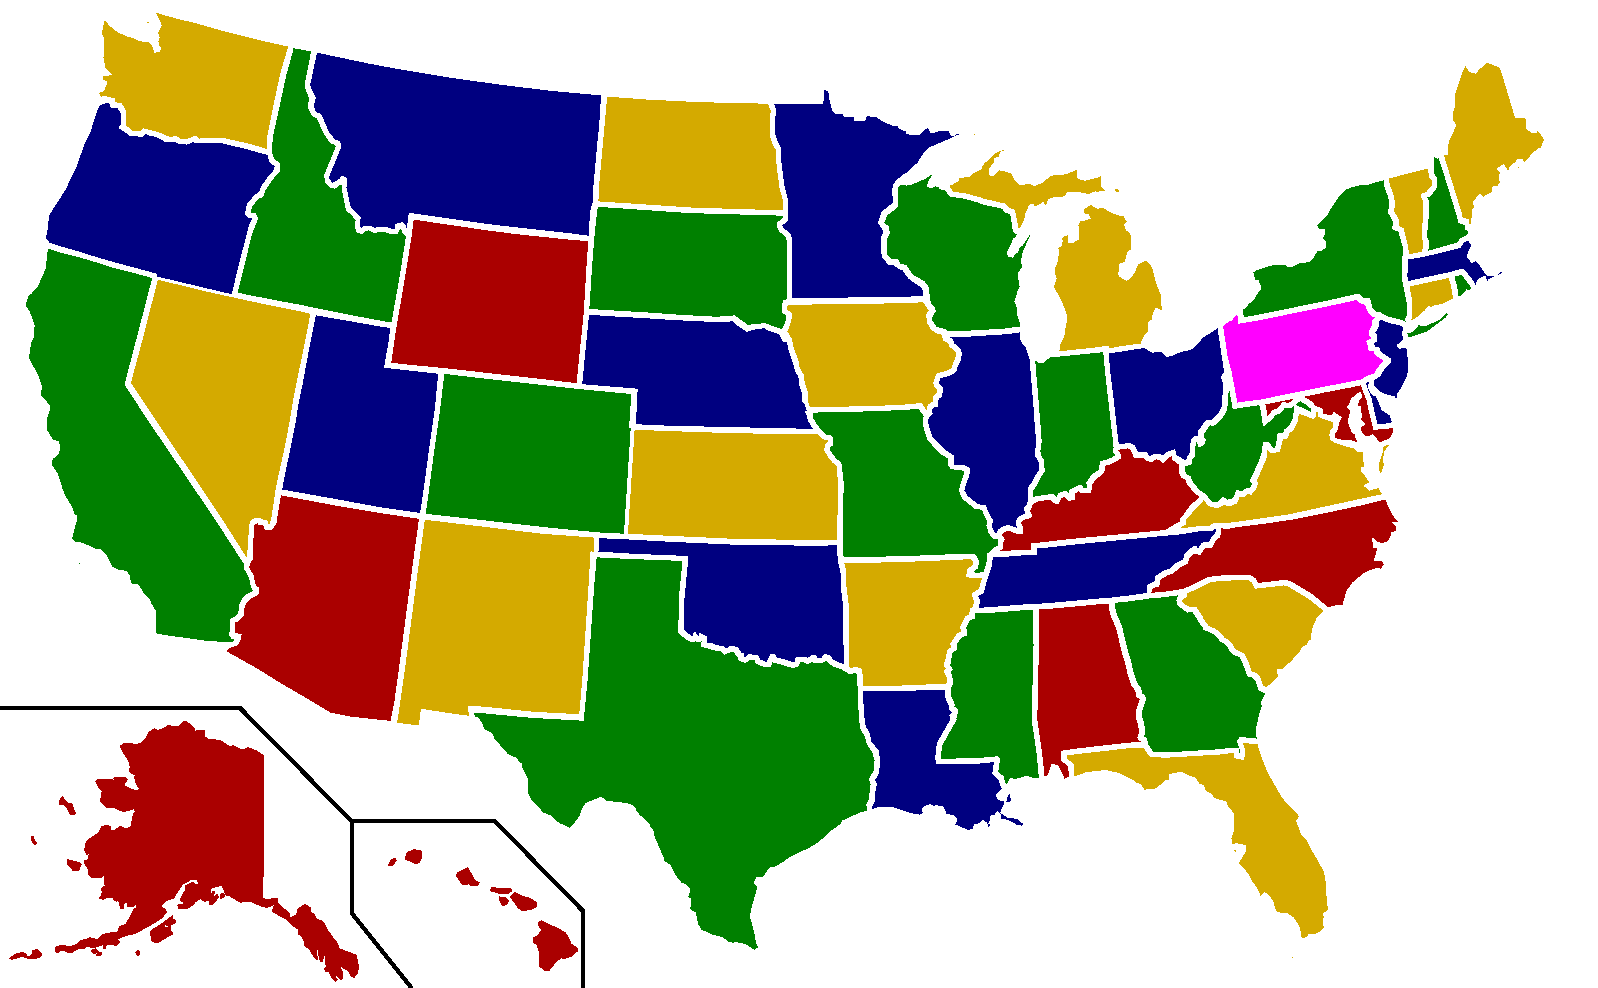
\includegraphics[width=\textwidth]{5color.pdf}
	\caption{Choose a nobe and color it different.}
	\end{subfigure}

	\begin{subfigure}[b]{0.45\textwidth}
	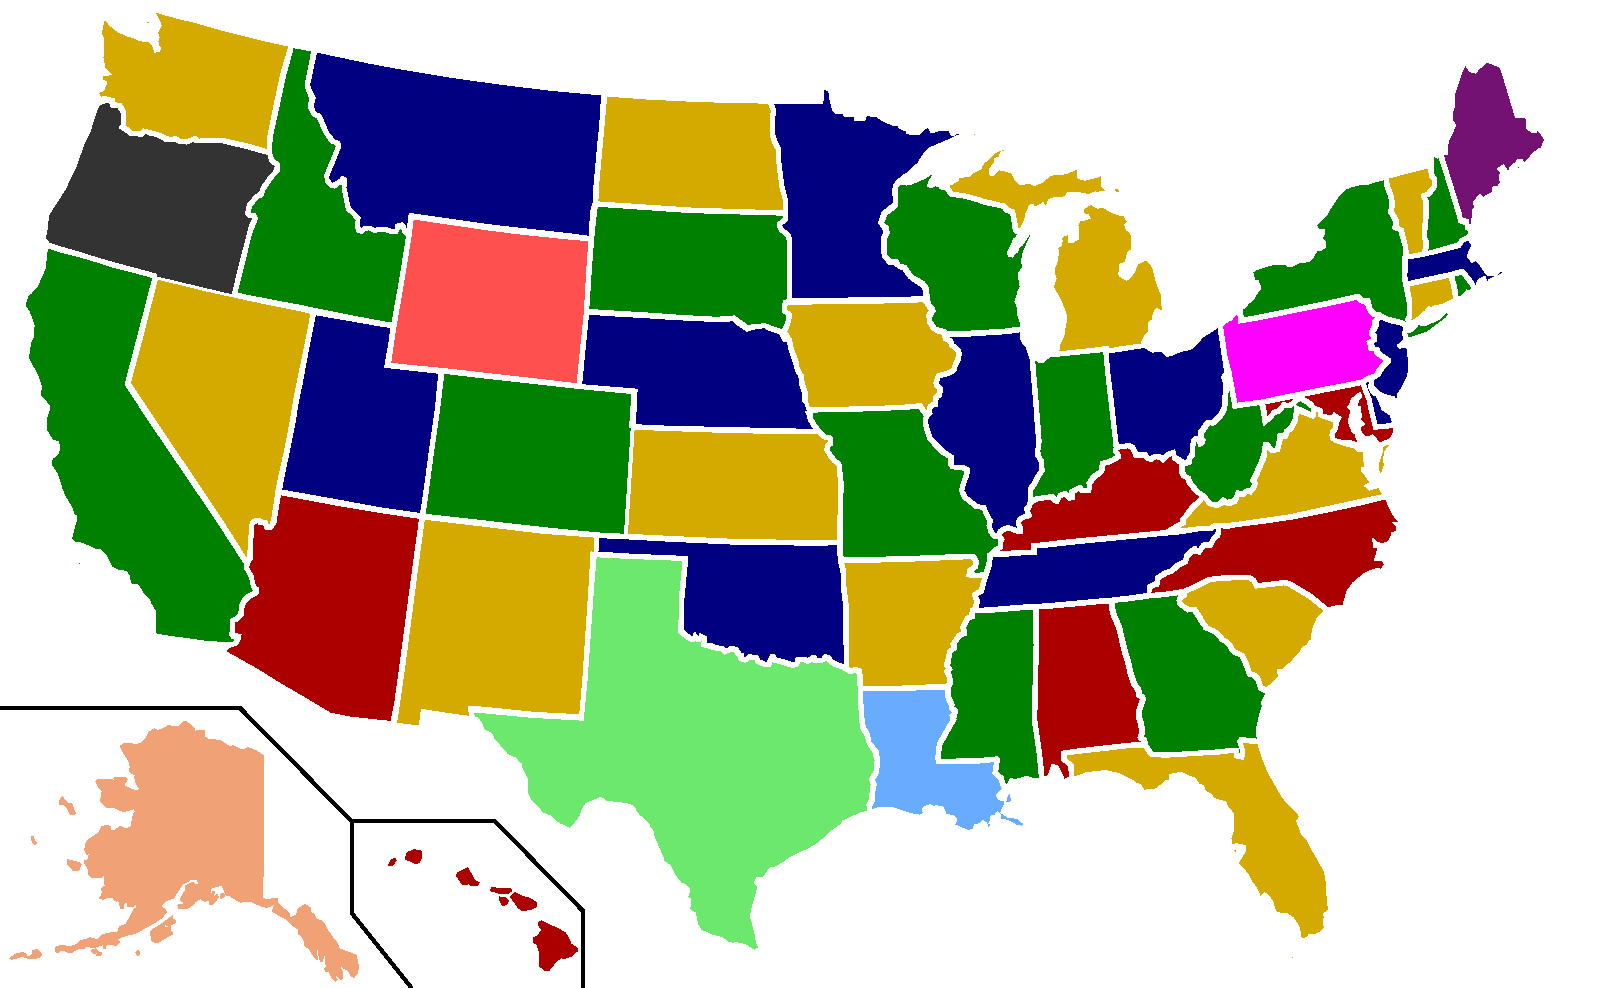
\includegraphics[width=\textwidth]{12color.pdf}
	\caption{Repeat that seven more times to get a 12-coloring! \\ \vspace{3.3em}}
	\end{subfigure}
	\quad
	\begin{subfigure}[b]{0.45\textwidth}
	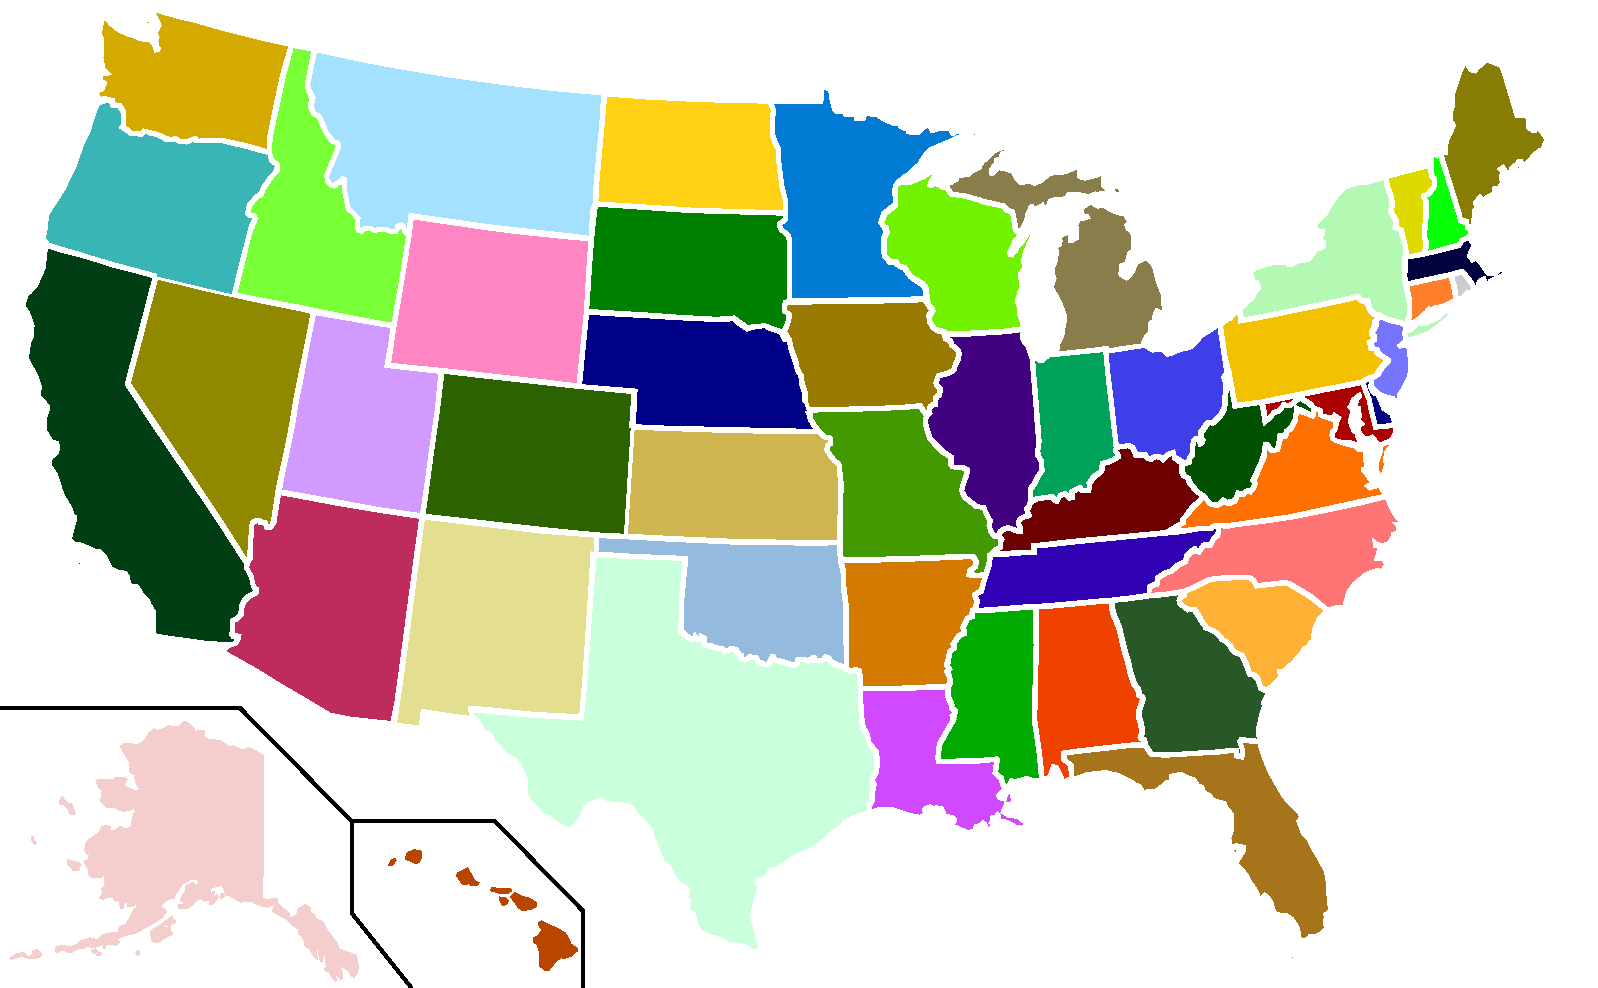
\includegraphics[width=\textwidth]{50color.pdf}
	\caption{If you had 51 different colors and wanted to use them all, it would look like this. However, a proof of the existence of generalized 51-colorings is left to future work.}
	\end{subfigure}
	\caption{Mr. Blum said we needed to have some pictures in our paper, so we pretended the USA was a graph and colored it like our algorithm says.}
	\label{fig:usa}
\end{figure}

\end{document}

